\documentclass[pdf]{beamer}
\mode<presentation>{}

\usetheme{Frankfurt}
\usepackage{listings}
\usepackage{color}
\usepackage{amsmath}
\usepackage{wasysym}
\usepackage{bm}

\usefonttheme[onlymath]{serif}

\newcommand\norm[1]{\left\lVert#1\right\rVert}

%% preamble
\title[Regularization]{Regularization in Deep Neural Networks}

\author{Paul Stey}
\date{March 3, 2017}

\begin{document}

%% title frame
\begin{frame}
\titlepage
\end{frame}



\begin{frame}<beamer>{Table of Contents}
	\tableofcontents[currentsection, 
				 currentsubsection, 
				 sectionstyle=show, 
				 subsectionstyle=show]
\end{frame}


\section{Introduction}
	\subsection{Regularization}
		\begin{frame}{What is Regularization?}
			\begin{center}
				Method of calibrating the complexity of our model  
			\end{center}
			
		\end{frame}
		
		
		\begin{frame}{What is Regularization?}
			\begin{enumerate}
				
				\item Very general (i.e., applicable to variety of models)
				\item Penalized regression
					\begin{enumerate} [1]
						\item Ridge regression
						\item Lasso 
						\item Elastic net
					\end{enumerate}
				\item XGBoost improvement on AdaBoost 
			\end{enumerate}
		\end{frame}	
	
		
		
	\subsection{Penalized Regression}
				
		\begin{frame}{$L_2$ Regularization Regression}
		\begin{enumerate}
			\item Ridge regression, also called Tikhonov regularization (Tikhonov, 1963)
			\item Penalize the $L_2$ norm 
			\item Constrains the Euclidian distance of $\beta$	
				\newline
				
				Given the linear model
				\vspace{-1.5em}
				\begin{center}
				$$ y_i = \beta_0 + \beta_1x_{i1} + \beta_2x_{i2} + ... + \beta_px_{ip} + \epsilon_i $$
				\end{center}
			
				the ridge penalty constrains
				$$ \norm{\beta}_2 = \sqrt{\beta_{1}^2 + \beta_{2}^2 + ... + \beta_{p}^2} $$
		\end{enumerate}
		\end{frame}
		
		
		\begin{frame}{$L_2$ Regularization cont.}
			Recall the least squares solution is obtained by
			\vspace{-1em}
			\begin{center}
				$$ \widehat{\beta} = \left(\bm{X}^T\bm{X}\right)^{-1} \bm{X}^Ty. $$
			\end{center}
			The ridge penalty gives us
			\vspace{-1em}
			\begin{center}
				$$ \widehat{\beta}^{ridge} = \left(\bm{X}^T\bm{X} + \lambda\bm{I}\right)^{-1} \bm{X}^Ty $$
			\end{center}
			\vspace{1em}
			where $\lambda$ is a penalty term, and $\bm{I}$ is the $p \times p$ identity matrix.
		\end{frame}
		
		
		\begin{frame}{$L_2$ Regularization cont.}
		\begin{enumerate}
			\item Penalty $\lambda$ is in the interval $\left[0, \infty \right)$
			\item Shrinks $\beta_j$ values towards $0$ (and each other)  
			\item Benefits: 
				\begin{enumerate}[1]
					\item Reduce model variance (i.e., more generalizable)
					\item Gain stability in estimates involving correlated data
					\item Computationally efficient
				\end{enumerate}
							
			\item Drawbacks:
				\begin{enumerate}[1] 
					\item Sacrifice unbiasedness of maximum likelihood estimate 
				\end{enumerate}
		\end{enumerate}
		\end{frame}
		
		\begin{frame}{$L_1$ Regularization}
		The lasso
		\begin{enumerate}
			\item Similar to ridge regression
			\item Penalize $L_1$ norm of $\beta$
			\item Constrains taxicab distance spanned by vector of regression coefficients
			$$ \norm{\beta}_1 = \left|\beta_{1}\right| + \left|\beta_{2}\right| + ... + \left|\beta_{p}\right| $$
			\item As $\lambda$ increases, $\beta_j \rightarrow 0$ 
				\begin{enumerate}[1]
					\item $\beta_j$ for less important predictors shrink faster
					\item Can be used for ``variable selection''
				\end{enumerate}
		\end{enumerate}
		\end{frame}

		\begin{frame}{Elastic Net}
		\begin{enumerate}
			\item Penalize \emph{both} the $L_1$ and ${L_2}$ norms of $\beta$
			\item Advantage of combining strengths of both approaches
		\end{enumerate}
		
		\vspace{2em} 
		
		\textit{Caveat}: Note that we often use ridge or lasso for very specific reason (i.e., ridge for accuracy, lasso for variable selection). One might suggest we give away this clarity of purpose when using the elastic net. 
		\end{frame}

\section{Broader View}
	\subsection{Non-Obvious Examples}
		\begin{frame}{Regularization More Broadly}
		Recall that regularization is merely a method of controlling model complexity. \newline 
		
		The standard shrinkage method examples make this very transparent with the use of explicit penalty terms. 
		\end{frame}	
		
		\begin{frame}{Broader View cont.}
		Consider less obvious examples: \newline
		
		\begin{enumerate}
			\item Number of boosting iterations 
			\item Learning rate for gradient descent 
			\item Bagging proportion
			\item Proportion in training \textit{vs}. test set
		\end{enumerate}
		\end{frame}		
	
		\begin{frame}{Broader View cont.}
		The essential feature of regularization is that it involves using some mechanism to control the complexity of our model. This makes our model more generalizable. 
		\end{frame}		
			
\section{Regularizing Neural Networks}
	\subsection{Norm Penalties}
	
	
	\subsection{Drop Out}
		
		\begin{frame}{Drop Out}
		\begin{enumerate}
			\item ...
		\end{enumerate}
		\end{frame}
		
		\begin{frame}{Compare with Random Forests}
		Consider similarities with random feature subset selection in random forests. \newline 
		
		 Both have a kind of ``thinning'' effect on model by using randomization to artificially restrict the parameters.   
		\end{frame}

	\subsection{Data Augmentation}
		
		\begin{frame}{Data Augmentation}
		\begin{enumerate}
			\item Adding [synthetic] data
			\item Or perturbing existing data 
			\item Or both!
			\item Similarities with 
		\end{enumerate}
		\end{frame}

		
		\begin{frame}{Data Augmentation Examples}
		\begin{enumerate}
			\item Translating images by a few pixels 
			\item Injecting noise in speech recognition data
		\end{enumerate}
		\end{frame}
		
	
	\subsection{Adversarial Training}
		
		\begin{frame}{Adversarial Training}
		\begin{enumerate}
			\item Szegedy \textit{et al.} 2014
			\item Similar in a sense to data augmentation
			\item Generate new observations in such a way as to maximize the chance they are misclassified
		\end{enumerate}
		\end{frame}
		
		\begin{frame}{Adversarial Training Example}
			\begin{figure}
				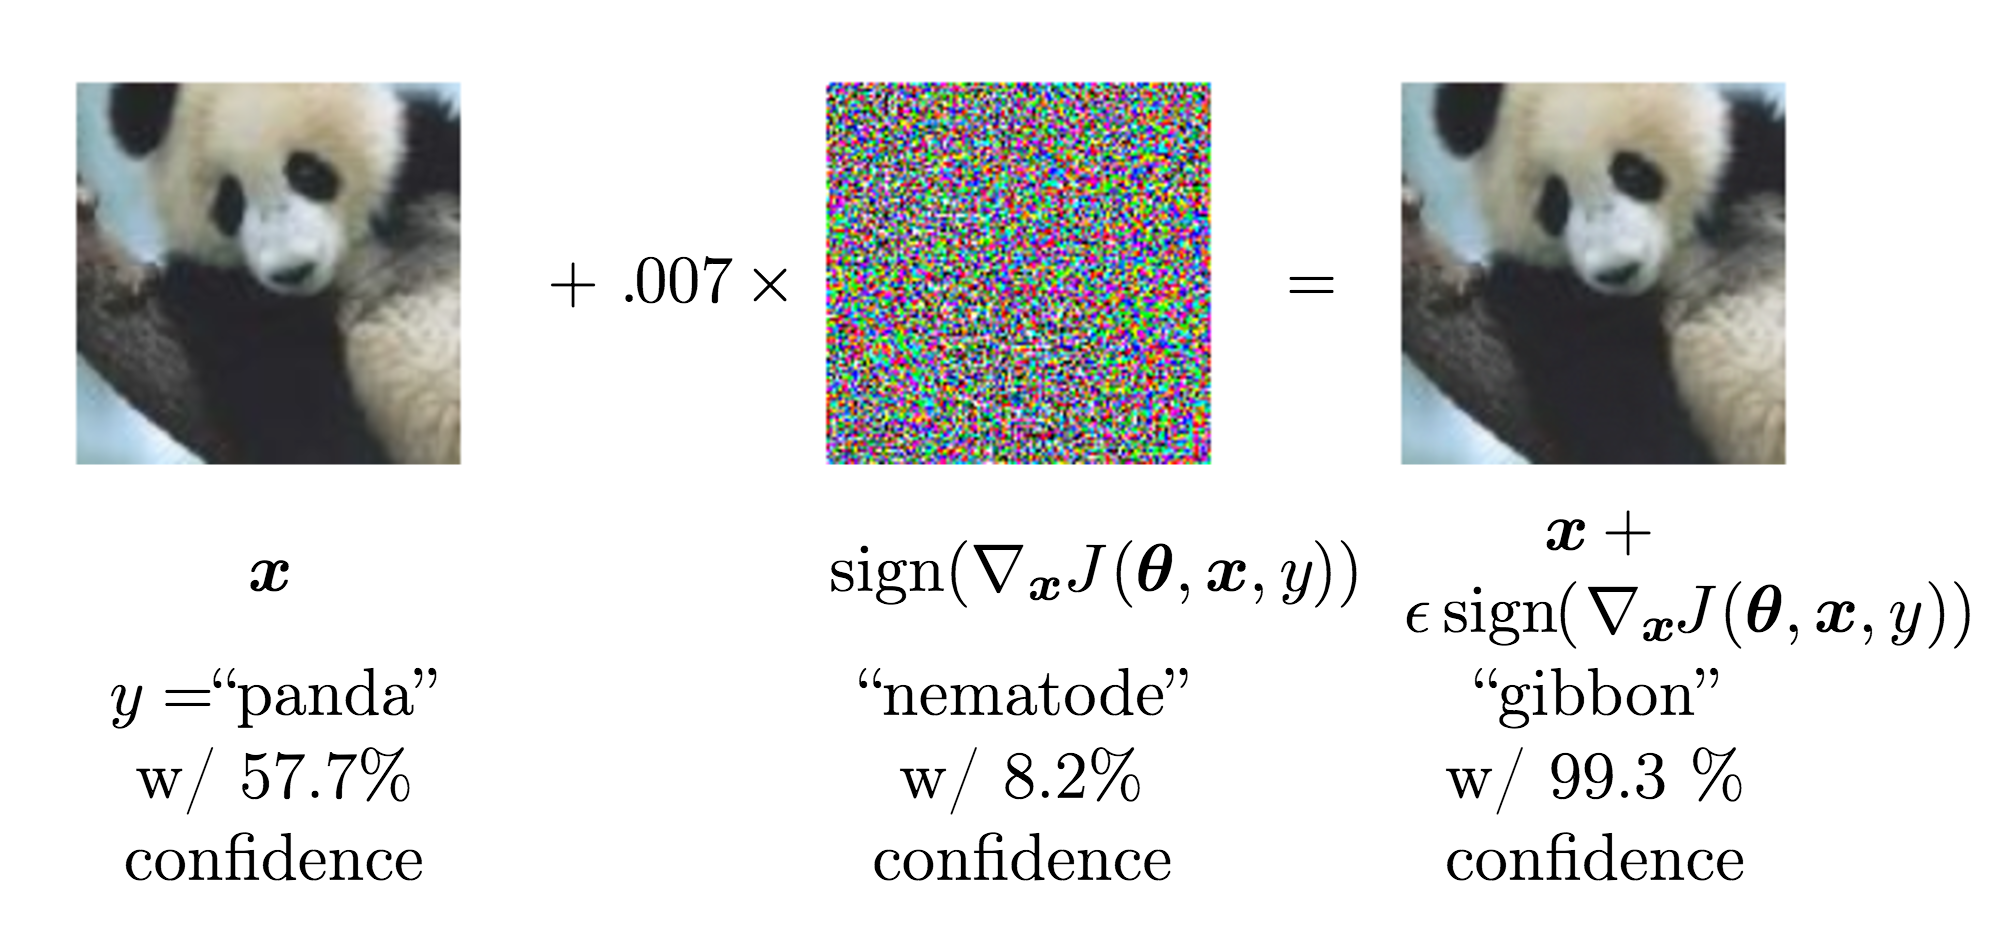
\includegraphics[scale = 0.25]{panda.png}
			\end{figure}		
    		\end{frame}
\section{Conclusion}
	\subsection{Summary}
	
	\subsection{Other Methods}
		
		\begin{frame}{Methods we Did Not Discuss}
			\begin{enumerate}
				\item Early stopping
				\item Bagging (Breiman, 1994)
				\item Parameter sharing (Laserre \textit{et al}., 2006)
			\end{enumerate}
		\end{frame}
\end{document}